\documentclass[8pt,hyperref={pdfpagelabels=true},xcolor=table,aspectratio=169]{beamer}
\usepackage[utf8]{inputenc}
\usepackage[T1]{fontenc}
\usepackage{helvet}
\usepackage{amsmath,amssymb,mathtools,amsfonts,bm,nicefrac}
\usepackage{tabularx}
\usepackage{booktabs}
\usepackage{setspace}
\usepackage{siunitx}
\usepackage{multicol}
\usepackage[absolute,overlay]{textpos}
\usepackage{colortbl}
\usepackage{array}
\usepackage{tikz}
\usetikzlibrary{shapes.geometric, arrows, positioning}

\DeclareMathOperator*{\argmax}{argmax}
\DeclareMathOperator*{\argmin}{argmin}
\DeclarePairedDelimiter\abs{\lvert}{\rvert}
\DeclarePairedDelimiter\norm{\lVert}{\rVert}

\definecolor{mygreen}{RGB}{0, 127, 0}
\definecolor{myred}{RGB}{127, 0, 0}
\definecolor{myblue}{RGB}{0, 0, 127}
\definecolor{mygrey}{RGB}{127, 127, 127}

% TikZ styles for flowcharts
\tikzstyle{io2} = [rectangle, rounded corners, minimum width=1.5cm, minimum height=1cm, align=center, draw=black, fill=gray!20]
\tikzstyle{process2} = [rectangle, minimum width=1.5cm, minimum height=1cm, align=center, draw=black, fill=blue!20]
\tikzstyle{investigate2} = [rectangle, very thick, rounded corners, minimum width=1.5cm, minimum height=1cm, align=center, draw=black, fill=orange!40]
\tikzstyle{arrow2} = [thick,->,>=stealth]

\renewcommand{\familydefault}{\sfdefault}

\title{Array Agnostic Low Latency DNN-Based\\ Online Source Counting}
\subtitle{SigProc Group Meeting}
\date{\today}
\author[Henri Gode]{\underline{Henri Gode}}
\hypersetup{pdfauthor={Henri Gode}}
\institute{Signal Processing Group}

\usetheme{uol}

\begin{document}

% ----------------------------------------------------------------------
% 1. Title Slide
% ----------------------------------------------------------------------
\begin{frame}
    \titlepage
\end{frame}

% ----------------------------------------------------------------------
% 2. Intro Slide (Motivation & Objective)
% ----------------------------------------------------------------------
% \begin{frame}{Motivation \& Objective}
%     \begin{columns}[T]
%         \begin{column}{0.5\textwidth}
%             \textbf{Motivation}
%             \begin{itemize}
%                 \item Modern audio devices (e.g. hearing aids, teleconferencing) should provide a benefit in highly dynamic acoustic scenarios with varying active speakers.
%                 \item \textbf{Advanced algorithms} (source separation, speech enhancement, DOA estimation) \textbf{require} the knowledge of \textbf{the current number of active sources}.
%                 \item Often multi-microphone data ($M \ge 2$), providing rich spatial information.
%             \end{itemize}
%         \end{column}
%         \begin{column}{0.5\textwidth}
%             \begin{alertblock}{Objective}
%                 Develop a \textbf{training-based ML model} to perform \textbf{online, frame-by-frame source counting} with low latency, highly robust against unseen array geometries and varying microphone counts.
%             \end{alertblock}
%         \end{column}
%     \end{columns}
% \end{frame}


\begin{frame}{Motivation}
  \begin{minipage}[c]{0.49\textwidth}
    \textbf{Acoustic Scenario:}
    \begin{itemize}
      \item \textbf{Randomly active speakers}, reverberation and background noise degrade speech quality and intelligibility.
    \end{itemize}
    \vspace{1em}

    \onslide<2->{
      \textbf{Motivation for Source Counting:}
      \begin{itemize}
        \item Assistive listening devices (e.g. binaural hearing aids) aim to enhance speech quality and intelligibility.
        \item Online algorithms (source localization, extraction \& separation) often require \textbf{knowing the current number of active sources}.
      \end{itemize}
    }
    \vspace{1em}

    \onslide<3->{
      \textbf{Our Focus}
      \begin{itemize}
        \item \textbf{DNN-based} source counting
        \item \textbf{Low latency} (frame-causal)
        \item \textbf{Geometry-agnostic} (arbitrary microphone array configurations)
      \end{itemize}
    }
  \end{minipage}
  \hfill
  \begin{minipage}[c]{0.49\textwidth}
    \onslide<1->{
      \begin{figure}
        \includegraphics[width=0.9\textwidth]{figures_new/scenario_plot.pdf}
        \label{fig:scenario}
      \end{figure}
      \begin{figure}
        \includegraphics[width=\textwidth]{figures_new/source_activity_timeline.pdf}
        \label{fig:timeline}
      \end{figure}
    }
  \end{minipage}

\end{frame}

% ----------------------------------------------------------------------
% 3. General System Overview
% ----------------------------------------------------------------------
\begin{frame}{General System Overview - Single Feature}
    \begin{minipage}{0.75\textwidth}
        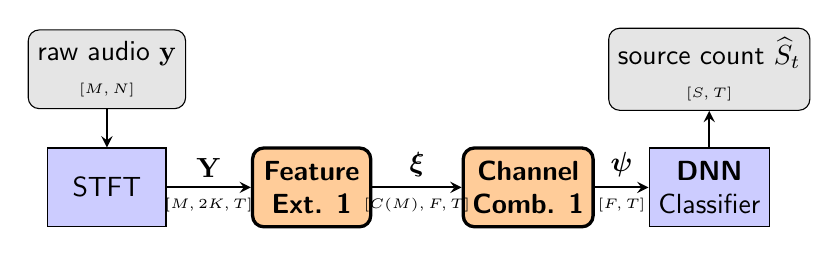
\begin{tikzpicture}

            % Place nodes
            \node (input) [io2] {raw audio $\mathbf{y}$\\ \tiny $\left[M, N\right]$};
            \node (stft) [process2, below of=input, node distance=1.5cm] {STFT};
            \node<2-> (feature) [investigate2, right of=stft, node distance=2.6cm] {\textbf{Feature} \\ \textbf{Ext. 1}};
            \node<3-> (chcombiner) [investigate2, right of=feature, node distance=2.75cm] {\textbf{Channel} \\ \textbf{Comb. 1}};
            \node<4-> (dnn) [process2, right of=chcombiner, node distance=2.3cm] {\textbf{DNN} \\ Classifier};
            \node<5-> (output) [io2, above of=dnn, node distance=1.5cm] {source count $\widehat{S}_t$ \\ \tiny $\left[S, T\right]$};

            % Draw edges
            \draw [arrow2] (input) -- (stft);
            % \draw [arrow2, dotted] (geometry) -| (dnn);
            \draw<2-> [arrow2] (stft) -- node[above] {$\mathbf{Y}$} node[below] {\tiny $\left[M, 2K, T\right]$} (feature);
            % \draw [arrow2] (stft) -- (feature);
            \draw<3-> [arrow2] (feature) -- node[above] {$\bm{\xi}$} node[below] {\tiny $\left[C(M),F,T\right]$} (chcombiner);
            \draw<4-> [arrow2] (chcombiner) -- node[above] {$\bm{\psi}$} node[below] {\tiny $\left[F,T\right]$} (dnn);
            \draw<5-> [arrow2] (dnn) -- (output);
        \end{tikzpicture}
    \end{minipage}
    \hfill
    \begin{minipage}{0.23\textwidth}
        \tiny
        \begin{itemize}
            \item $M \rightarrow$ \# microphones 
            \item $N \rightarrow$ \# time-samples 
            \item<2-> $T \rightarrow$ \# time-frames (STFT)
            \item<2-> $K \rightarrow$ \# frequencies (STFT)
            \item<3-> $C(M) \rightarrow$ \# channels 
            \item<3-> $F \rightarrow$ \# features
            \item<5-> $S \rightarrow$ max. \# sources
            \item<5-> $\widehat{S}_t \rightarrow$ estimated source count (at time $t$)
        \end{itemize}
    \end{minipage}

        \vspace{1.5em}
    \begin{itemize}
        \item \textbf{Frame-Causal Pipeline:} Processes data frame-by-frame without future lookahead.
        \item \textbf{Modularity:} Allows systematic ablation of feature extractors, combinators
    \end{itemize}
\end{frame}



% ----------------------------------------------------------------------
% 4. Details: Raw Audio & STFT
% ----------------------------------------------------------------------
\begin{frame}{Details: Raw Audio \& STFT}
    \begin{tikzpicture}[remember picture, overlay]
        \node[anchor=north east, xshift=-0.1cm, yshift=-0.1cm] at (current page.north east) {
            \includegraphics[width=0.60\textwidth]{figures_J3/flow_chart.png}
        };
    \end{tikzpicture}
    \underline{\textbf{Raw Audio Input}}
    \vspace{1.0em}
    \begin{itemize}
        \item Microphone signal array: $\mathbf{y} \in \mathbb{R}^{M \times N}$
        \item \textbf{Sampling Frequency:} $f_s = 8000$ Hz
        \item \textbf{Number of microphones:} $M \in [2, 8]$
        \item \textbf{Signal Length:} $\SI{120}{s} \rightarrow N = \SI{960000}{samples}$ \
    \end{itemize}
    \vspace{2em}
    \underline{\textbf{Short-Time Fourier Transform (STFT)}}
    \vspace{1.0em}
    \begin{itemize}
        \item \textbf{Frame Length:} $\SI{32}{\milli\second} \rightarrow N_{FFT} = 256$ samples
        \item \textbf{Frame Shift:} $\SI{16}{\milli\second} \rightarrow 128$ samples
        \item \textbf{Window Type:} square-root Hann
        \item \textbf{Frequency Bins:} $K = \frac{N_{FFT}}{2} + 1 = 257$ bins
        \item \textbf{Number of frames:} $T = \lceil \frac{N_{samples}}{128} \rceil + 1 = 7501$
        \item \textbf{STFT Output:} $\mathbf{Y} \in \mathbb{C}^{M \times K \times T} \rightarrow \mathbf{Y} \in \mathbb{R}^{M \times 2K \times T}$
    \end{itemize}
\end{frame}


% ----------------------------------------------------------------------
% 6. Details: Spectral Features
% ----------------------------------------------------------------------
\begin{frame}{Features}
    \begin{tikzpicture}[remember picture, overlay]
        \node[anchor=north east, xshift=-0.1cm, yshift=-0.1cm] at (current page.north east) {
            \includegraphics[width=0.6\textwidth]{figures_J3/flow_chart.png}
        };
    \end{tikzpicture}
    
    \onslide<1->{
        \begin{minipage}{0.4\textwidth}
            \vspace{-3em}
            \begin{block}{\textbf{Feature types}}
                \begin{itemize}
                    \item Spectral features
                    \item Spatial features
                    \item Microphone positions (relative)
                \end{itemize}
            \end{block}
        \end{minipage}
    }   
    \onslide<2->{
        \vspace{2em}
        \begin{itemize}
            \item \textbf{Raw STFT Features} (spectral \& spatial)
                  \begin{itemize}
                      \item $\bm{\xi}^{(STFT)} \in \mathbb{R}^{M \times 2K \times T}$
                      \item real \& imag (or magnitude \& phase)
                      \item \textit{Pros:} No information loss, still contains spatial information
                      \item \textit{Cons:} Highly dependent on geometry and very high dimensionality
                  \end{itemize}
              \vspace{1em}  
        \item \textbf{Log-Mel Features} (spectral)
              \begin{itemize}
                  \item $\bm{\xi}^{(Mel)} \in \mathbb{R}^{M \times K_{Mel} \times T}$
                  \item Nonlinear filterbank performs per-channel dim. reduction  \\ ($K=257$ freq. bins $\rightarrow K_{Mel}=80$ perceptual bands)
                  \item \textit{Pros:} Reduces dimensionality motivated by psychoacoustics
                  \item \textit{Cons:} Loss of spatial information
              \end{itemize}
    \end{itemize}
    }
\end{frame}

% ----------------------------------------------------------------------
% 7. Details: Spatial Features
% ----------------------------------------------------------------------
\begin{frame}{Details: Spatial Features}
    \begin{tikzpicture}[remember picture, overlay]
        \node[anchor=north east, xshift=-0.1cm, yshift=-0.1cm] at (current page.north east) {
            \includegraphics[width=0.6\textwidth]{figures_J3/flow_chart.png}
        };
    \end{tikzpicture}
    
    \onslide<1->{
        \begin{minipage}{0.4\textwidth}
            \vspace{-3em}
            \begin{block}{\textbf{Feature types}}
                \begin{itemize}
                    \item Spectral features
                    \item Spatial features
                    \item Microphone positions (relative)
                \end{itemize}
            \end{block}
        \end{minipage}
    }
    \onslide<1->{   
    \begin{itemize}
        \item \textbf{Inter-channel Phase Differences (IPD / CSIPD)} (spatial)
              \begin{itemize}
                  \item IPD: ${\Delta\phi_{ij}} = \phi_i - \phi_j \quad\rightarrow\quad \bm{\xi}_{t,f}^{(IPD)} \in \mathbb{R}^{P \times K \times T}$
                  \item CSIPD: Cosine and Sine of IPD \\ ${\Delta\phi_{ij}^{\text{cos}}} = \cos(\Delta\phi_{ij}), {\Delta\phi_{ij}^{\text{sin}}} = \sin(\Delta\phi_{ij}) \quad\rightarrow\quad \bm{\xi}_{t,f}^{(CSIPD)} \in \mathbb{R}^{2P \times K \times T}$
                  \item Number of pairs $P = \frac{M(M-1)}{2}$. For $M=8$, $P=28$.
              \end{itemize}
              \vspace{1em}
        \item \textbf{Generalized Magnitude Squared Coherence (GMSC \& wGMSC)} (spatial)
              \begin{itemize}
                  \item $\bm{\xi}_{t,f}^{(wGMSC)} \in \mathbb{R}^{1 \times 2KF \times T}$
                  \item Quantifies spatial coherence without explicit pairing; detects rank-1 covariance updates.
                  \item Whitened GMSC (wGMSC) focuses on \textit{change detection} (source activations/deactivations).
                  \item \textit{Pros:} Naturally aggregates $M$ channels into a single dimension! Independent of $M$.
              \end{itemize}
    \end{itemize}
    }
\end{frame}

% ----------------------------------------------------------------------
% 8. Details: Microphone Positions
% ----------------------------------------------------------------------
\begin{frame}{Details: Microphone Positions}

    \onslide<1->{
        \begin{block}{\textbf{Feautre types}}
            \begin{itemize}
                \item Spectral features
                \item Spatial features
                \item Microphone positions (relative)
            \end{itemize}
        \end{block}
    }   
    \onslide<2->{

    \textbf{Explicit Geometric Conditioning}
    \begin{itemize}
        \item Provide the neural network with the exact Cartesian coordinates of the active microphones relative to the array center.
        \item \textbf{Dimensions:} $\mathbf{G} \in \mathbb{R}^{M \times 3}$ (representing relative$x, y, z$ positions).
    \end{itemize}
    }
\end{frame}

% ----------------------------------------------------------------------
% 9. Details: Channel Combinators
% ----------------------------------------------------------------------
\begin{frame}{Details: Channel Combinators}
    To process an arbitrary number of microphones $M$ (or pairs $P$) through a fixed-size classifier, we must condense the spatial dimension to a fixed size $J$:
    \vspace{0.5em}
    \begin{enumerate}
        \item \textbf{Mean Pooling / Zero Padding}
              \begin{itemize}
                  \item Average over $M$, or pad with zeros up to $M_{max} = 8$.
                  \item \textit{Baseline approach.}
              \end{itemize}
        \item \textbf{TAC Layers (Transform-Average-Concatenate)}
              \begin{itemize}
                  \item Standard invariant approach for multi-channel processing in source separation.
              \end{itemize}
        \item \textbf{Self-Attention Channel Combination}
              \begin{itemize}
                  \item Permutation-invariant attention mechanism treating channels as a sequence.
              \end{itemize}
        \item \textbf{Cross-Attention (Global-to-Local Context)}
              \begin{itemize}
                  \item A global learned query vector attends to the individual local channel features.
              \end{itemize}
    \end{enumerate}
\end{frame}

% ----------------------------------------------------------------------
% 10. Details: Stacking / Fusion / Conditioning
% ----------------------------------------------------------------------
\begin{frame}{Details: Feature Stacking, Fusion \& Conditioning}
    \textbf{How do we unite Spatial, Spectral, and Coordinate Features?}
    \vspace{0.5em}
    \begin{itemize}
        \item \textbf{Basic Stacking (Our Baseline)}
              \begin{itemize}
                  \item Extract features $\rightarrow$ independently condense to fixed dimensions $J_{spatial}$ and $J_{spectral}$ $\rightarrow$ concatenate along the feature dimension before passing to the classifier.
              \end{itemize}
              \vspace{0.5em}
        \item \textbf{FiLM Layers (Feature-wise Linear Modulation)}
              \begin{itemize}
                  \item Use one feature (e.g., explicit microphone coordinates) to generate affine transformation parameters (shift and scale) applied to the acoustic features.
              \end{itemize}
              \vspace{0.5em}
        \item \textbf{Attention-Based Fusion}
              \begin{itemize}
                  \item Cross-attention between modalities deeper in the network.
              \end{itemize}
    \end{itemize}
\end{frame}

% ----------------------------------------------------------------------
% 11. Details: Source Count Estimation Classifier
% ----------------------------------------------------------------------
\begin{frame}{Details: Source Count Estimation Classifier}
    \textbf{Temporal Modeling Architecture}
    \begin{itemize}
        \item \textbf{Default Model:} Transformer sequence-to-sequence classifier.
        \item \textit{Alternatives open for investigation:} Recurrent Neural Networks (RNN/GRU), Temporal Convolutional Networks (TCN), Conformers.
    \end{itemize}
    \vspace{1em}
    \textbf{Classification Output}
    \begin{itemize}
        \item Softmax layer across discrete source count classes.
        \item Maximum simulated sources: $K_{max} = 4$.
        \item Total Output Classes: $5$ (Counts: $0, 1, 2, 3, 4$).
        \item \textbf{Inference:} The framewise source count estimate $\widehat{K}_t$ is derived via the $\argmax$ operation over the class probabilities at each frame.
    \end{itemize}
\end{frame}


% ----------------------------------------------------------------------
% 12. General System Overview - Multi-Feature Fusion
% ----------------------------------------------------------------------
\begin{frame}{General System Overview - Multi-Feature Fusion}
    \begin{center}
        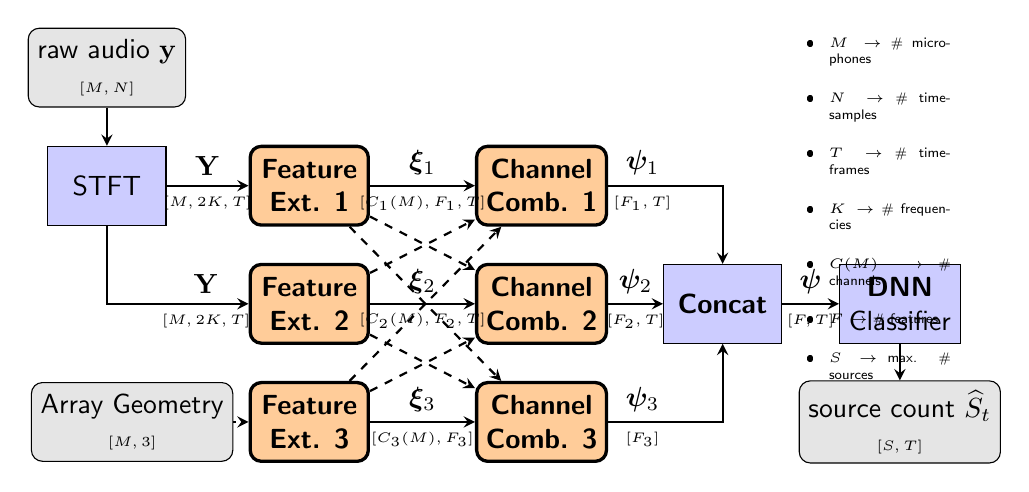
\begin{tikzpicture}

            % Place nodes
            \node (input) [io2] {raw audio $\mathbf{y}$\\ \tiny $\left[M, N\right]$};
            \node (stft) [process2, below of=input, node distance=1.5cm] {STFT};
            \node (feature) [investigate2, right of=stft, node distance=2.57cm] {\textbf{Feature} \\ \textbf{Ext. 1}};
            \node (feature2) [investigate2, below of=feature, node distance=1.5cm] {\textbf{Feature} \\ \textbf{Ext. 2}};
            \node (feature3) [investigate2, below of=feature2, node distance=1.5cm] {\textbf{Feature} \\ \textbf{Ext. 3}};
            \node (chcombiner) [investigate2, right of=feature, node distance=2.95cm] {\textbf{Channel} \\ \textbf{Comb. 1}};
            \node (chcombiner2) [investigate2, right of=feature2, node distance=2.95cm] {\textbf{Channel} \\ \textbf{Comb. 2}};
            \node (chcombiner3) [investigate2, right of=feature3, node distance=2.95cm] {\textbf{Channel} \\ \textbf{Comb. 3}};
            \node (geometry) [io2, left of=feature3, node distance=2.25cm] {Array Geometry \\ \tiny $[M, 3]$};
            \node (stacker) [process2, right of=chcombiner2, node distance=2.3cm] {\textbf{Concat}};
            \node (dnn) [process2, right of=stacker, node distance=2.25cm] {\textbf{DNN} \\ Classifier};
            \node (output) [io2, below of=dnn, node distance=1.5cm] {source count $\widehat{S}_t$ \\ \tiny $\left[S, T\right]$};  

            % Draw edges
            \draw [arrow2] (input) -- (stft);
            \draw [arrow2, dotted] (geometry) -- (feature3);
            % \draw [arrow2, dotted] (geometry) -| (dnn);
            \draw [arrow2] (stft) -- node[above] {$\mathbf{Y}$} node[below] {\tiny $\left[M, 2K, T\right]$} (feature);
            % \draw [arrow2] (stft) -- (feature);
            \draw [arrow2] (stft) |- node[above, pos = 0.85] {$\mathbf{Y}$} node[below, pos = 0.85] {\tiny $\left[M, 2K, T\right]$} (feature2);
            % \draw [arrow2] (stft) |- (feature2);
            \draw<2-> [arrow2, dashed] (feature) -- (chcombiner2);
            \draw<2-> [arrow2, dashed] (feature) -- (chcombiner3);
            \draw<2-> [arrow2, dashed] (feature2) -- (chcombiner);
            \draw<2-> [arrow2, dashed] (feature2) -- (chcombiner3);
            \draw<2-> [arrow2, dashed] (feature3) -- (chcombiner2);
            \draw<2-> [arrow2, dashed] (feature3) -- (chcombiner);
            \draw [arrow2] (feature) -- node[above] {$\bm{\xi}_1$} node[below] {\tiny $\left[C_1(M),F_1,T\right]$} (chcombiner);
            \draw [arrow2] (feature2) -- (chcombiner2);
            \path<1> (feature2) -- node[above] {$\bm{\xi}_2$} node[below] {\tiny $\left[C_2(M),F_2,T\right]$} (chcombiner2);
            \draw [arrow2] (feature3) -- node[above] {$\bm{\xi}_3$} node[below] {\tiny $\left[C_3(M),F_3\right]$} (chcombiner3);
            \draw [arrow2] (chcombiner) -| node[above, pos=0.15] {$\bm{\psi}_1$} node[below, pos=0.15] {\tiny $\left[F_1,T\right]$} (stacker);
            \draw [arrow2] (chcombiner2) -- node[above] {$\bm{\psi}_2$} node[below] {\tiny $\left[F_2,T\right]$} (stacker);
            \draw [arrow2] (chcombiner3) -| node[above, pos=0.15] {$\bm{\psi}_3$} node[below, pos=0.15] {\tiny $\left[F_3\right]$} (stacker);
            \draw [arrow2] (stacker) -- node[above] {$\bm{\psi}$} node[below] {\tiny $\left[F,T\right]$} (dnn);
            \draw [arrow2] (dnn) -- (output);
            
            % Legend in the upper right corner
            \node (legend) [anchor=north east] at (dnn.east |- input.north) {
                \begin{minipage}{0.2\textwidth}
                    \tiny
                    \begin{itemize}
                        \item $M \rightarrow$ \# microphones 
                        \item $N \rightarrow$ \# time-samples 
                        \item $T \rightarrow$ \# time-frames 
                        \item $K \rightarrow$ \# frequencies 
                        \item $C(M) \rightarrow$ \# channels 
                        \item $F \rightarrow$ \# features
                        \item $S \rightarrow$ max. \# sources
                    \end{itemize}
                \end{minipage}
            };
        \end{tikzpicture}
    \end{center}
    \vspace{1.5em}
    \begin{itemize}
        \item \textbf{Causal Pipeline:} Processes data frame-by-frame without future lookahead.
        \item \textbf{Modularity:} Allows systematic ablation of feature extractors, combinators, and fusion schemes.
    \end{itemize}
\end{frame}

% ----------------------------------------------------------------------
% 12. Experiments Part 0: The Role of Spatial Features
% ----------------------------------------------------------------------
\begin{frame}{Scientific Questions -- Part 0: Role of Spatial Features}
    \begin{block}{Question}
        Does the explicit integration of spatial information yield a quantifiable benefit over pure spectral processing for source counting?
    \end{block}
    \vspace{1em}
    \textbf{Approach \& Expectation:}
    \begin{itemize}
        \item Compare systems utilizing:
              \begin{enumerate}
                  \item Spectral features only
                  \item Spatial features only
                  \item Combined Spectral + Spatial features
              \end{enumerate}
        \item We strongly expect that additional spatial information leads to substantially improved performance.
        \item This serves as our foundational baseline, corroborated by existing literature (e.g., Cornell baseline paper).
    \end{itemize}
\end{frame}

% ----------------------------------------------------------------------
% 13. Experiments Part 1: Robustness to Array Geometries
% ----------------------------------------------------------------------
\begin{frame}{Scientific Questions -- Part 1: Robustness to Array Geometries}
    \begin{block}{Question}
        How does performance drop during inference when using an unseen array (different geometry or differing number of microphones)?
    \end{block}
    \vspace{1em}
    \textbf{The $4 \times 4$ Evaluation Matrix}
    \begin{itemize}
        \item We hypothesize that GMSC-based features abstract spatial properties more effectively and are thus more robust to geometric variations.
        \item \textbf{Setup:} We generate 4 independent synthetic training datasets with distinct characteristics.
        \item We train 4 individual systems and evaluate each against all 4 test sets.
    \end{itemize}
    \vspace{1em}
    \begin{center}
        \begin{tabular}{l|c|c}
            \toprule
            \textbf{Training Set Variants} & \textbf{Fixed 8-Channels} & \textbf{Variable 2-8 Channels} \\
            \midrule
            \textbf{Circular Geometry}     & Dataset 1                 & Dataset 3                      \\
            \textbf{Random Geometry}       & Dataset 2                 & Dataset 4                      \\
            \bottomrule
        \end{tabular}
    \end{center}
\end{frame}

% ----------------------------------------------------------------------
% 14. Experiments Part 2: Conditioning with Relative Mic Positions
% ----------------------------------------------------------------------
\begin{frame}{Scientific Questions -- Part 2: Conditioning with Mic Positions}
    \begin{block}{Question}
        Can explicit architectural awareness of the physical microphone layout bridge the performance gap on unseen arrays?
    \end{block}
    \vspace{1em}
    \textbf{Approach:}
    \begin{itemize}
        \item Append the relative exact positions of the microphones ($\mathbf{G} \in \mathbb{R}^{M \times 3}$) as an explicit auxiliary feature stream.
        \item Analyze how this specific conditioning improves overall robustness.
        \item \textbf{Primary Focus:} Utilizing the whitened Generalized Magnitude Squared Coherence (wGMSC) as the core spatial feature, given its natural summarization properties and proven capability for change detection.
    \end{itemize}
\end{frame}

% ----------------------------------------------------------------------
% 15. Datasets Configuration
% ----------------------------------------------------------------------
\begin{frame}{PRA-ANF Datasets Configuration}
    \textbf{Simulated Dataset Parameters (PRA-ANF Base)}
    \begin{itemize}
        \item \textbf{Scale:} Train = 2400 scenarios, Val = 300 scenarios, Test = 300 scenarios.
        \item \textbf{Scenario Length:} $60.0$ seconds.
        \item \textbf{Maximum Sources:} $4$ simultaneous or sequential speakers.
        \item \textbf{Acoustics:} Simulated via PyRoomAcoustics (PRA) with dynamic Spatial Anisotropic Noise Fields (ANF).
        \item \textbf{Signal-to-Noise Ratios (SNR):} Uniformly distributed between $5.0$ and $20.0$ dB.
        \item \textbf{Source Dynamics:} Random activations, with silence lengths and voice activity detection explicitly defining Oracle Ground Truth overlaps.
    \end{itemize}
    \vspace{1em}
    \textit{(Open for discussion: Should we scale training up to 4800 scenarios for final production?)}
\end{frame}

% ----------------------------------------------------------------------
% 16. Summary
% ----------------------------------------------------------------------
\begin{frame}{Summary}
    \begin{itemize}
        \item \textbf{The Goal:} A causal, real-time source count estimator robust to unknown array configurations.
        \item \textbf{The Architecture:} A highly modular STFT-based pipeline processing heterogeneous features through specific channel combinators into a Transformer sequence classifier.
        \item \textbf{The Roadmap:}
              \begin{itemize}
                  \item \textbf{Part 0:} Confirm benefit of combined spatial + spectral features.
                  \item \textbf{Part 1 ($4\times4$ matrix):} Quantify performance degradation on unseen arrays across Circular/Random and Fixed/Variable constraints.
                  \item \textbf{Part 2:} Inject explicit array coordinate conditioning to recover performance on generalization tasks.
              \end{itemize}
    \end{itemize}
    \vspace{2em}
    \begin{center}
        \textbf{Thank You!} \\
        Questions \& Discussion
    \end{center}
\end{frame}

\end{document}
